\chapter{Análise Bibliográfica sobre Sistemas de Informação em transporte ...\label{chap:bibliometria:MoustacheGolem}}


\section{Planejamento do estudo}

Sonhos e ambições humanas relacionadas a transporte sempre frequentemente envolvem voo, afinal quem não se imaginou obtendo liberdade absoluta através de asas. De certa forma essa ambição foi conquistada a décadas, mas de forma limitada pois o carro voador não foi inventado ainda, assim esse continua sendo um sonho de meio de transporte. O desenvolvimento e popularidade de inteligência adicionou outra ambição de transporte, o carro auto condutor, desenvolvimento desse se encontra relativamente avançado. 

Mas, esses não são os únicos caminhos promissores evolução do transporte, sistemas de informação, Sendo esses sistemas que utilizam hardware e software para aplicações utilizando grande quantia de informações, afetaram bastante o desenvolvimento de tecnologia na saúde e negócios, aqui vou tentar explorar pesquisas de sistemas de informação em torno de transportes.


\begin{itemize}
    

\item Qual a base de conhecimentos científicos produzida em torno do tema
Sistemas de informação em transporte


\item Quais os principais termos e conceitos ligados à frente de pesquisa no tema sistemas de informação em transporte.

\item Como a sistemas de informação tem sido usado para alterar tecnologias de transporte.

\item Qual a estrutura social da comunidade, se é que existe, que pesquisa
sobre o tema de sistema de informação em transporte.
\end{itemize}

\subsection{O que já existe de pesquisa bibliométrica sobre
esse tema?}
O tema de transporte mais generalizado possui varias pesquisas, algumas explorando décadas e décadas de bibliografia, mas \cite{cobo_bibliometric_2013} é a que mais se aproxima do que temos como alvo.


\subsection{Uso do Bibliometrix e Biblioshiny}
Também serão usadas a ferramenta e o workflow proposto pelos autores do pacote Bibliometrix.

\subsection{Limitações} O exercício relatado foi feito em menos de uma semana, envolvendo  provavelmente mais de 10 horas, em meio a limitações impostas por outros estudos.
%%%%%%%%%%%%%%%%%%%%%%%%%%%%%%%%%%%%%%%%%%%%%%%%%%%%%%%%%%
\newpage
\section{Coleta de dados}

A coleta de dados feita usando o WoS no dia 09 de fevereiro de 2022, acessado por meio do Portal de Periódicos da CAPES.

Foram feitas buscas nas coleções Science  Citation  Index  Expanded (SCI -EXPANDED) e Social  Sciences  Citation  Index (SSCI).

\subsection{Explicação dos termos de busca:}
Todas as queries foram efetuadas tendo \textbf{Tópicos} como alvo.
\begin{itemize}

\item A primeira versão da query utilizada foi

\begin{verbatim}
    1   transportation and information systems
\end{verbatim}

Uma busca simples, mas buscar por palavras tão abrangentes
quanto
\textit{information} e \textit{systems} gera resultados explorando
temas completamente separados do que temos como alvo.

\item A segunda versão da query utilizada foi:

\begin{verbatim}
    1   transport* and (information system*)
\end{verbatim}


Nesse ponto não havia entendido os resultados osuficiente para
Entender \newline a abrangência causado pelos termos \textit{information} e
\textit{systems}, mas utilizar \textit{transport*} ajudou a puxar
resultados mais relevantes.


\item A ultima versão da query utilizada foi:

\begin{verbatim}
    1   transport* and (information-system*)
\end{verbatim}


Na ultima query também foi utilizado o filtro de categoria da WoS:
\begin{verbatim}
    1   Transportation science technology
\end{verbatim}

Que focou bastante os resultados em exatamente o que queríamos.
Ainda assim escolhi continuar a limitar os resultados com o termo \textit{transport*}, pois ele ainda ajuda a focar os resultados, sem ele ajuda a eliminar por exemplo pesquisas tangenciais a transporte, como por exemplo, pesquisas em embarcados.

\textit{information-system*} finalmente possui um \emph{-}, que foca os resultados no campo de estudo alvo.

Os 1731 registros obitidos estão localizados em \url{https://github.com/jhcf/Comput-Experim-20212/experiments/MoustacheGolem/T1/0902records.txt}

Foram utilizadas as opções Exportar registros para arquivo de texto \newline sem formatação,  e o conteúdo gravado foi \textit{Registro completo e Referencias citadas}
Os 1728 registros foram recuperados em 5
blocos de até 500 registros por vez (1-500, 501-1000, 1001-1500, 
1501-1731).

A formatação de 127 linhas de um registro no formato RIS, referentes a um artigo recuperado da Web of Science pode ser encontrada descrita em mais detalhes em \citep{wikipedia_ris_2017}.

\end{itemize}

%%%%%%%%%%%%%%%%%%%%%%%%%%%%%%%%%%%%%%%%%%%%%%%%%%%%%%%%%%
\section{Análise dos dados}

\subsection{Filtragem de registros}

Foi aplicado um filtro ao dataset  inicial, com 1731 registros, que continham pŕevias de artigos, artigos de conferência, capítulos de livro etc. Foram mantidos apenas os registros de artigos publicados em revistas científicas. Após a aplicação desse filtro, 1274 registros foram mantidos no dataset, chamarei esses de DSF(dataset filtrado).

\subsection{Análise descritiva do DSF}


As informações mais gerais sobre o DSF são as seguintes:
\begin{description}
    \item [\textit{Timespan}] Os artigos que atenderam aos critérios de busca e filtragem foram publicados a partir de 1977, até 2022. Assim, não foram encontrados registros entre 1945 e 1976.
    
    \item [\textit{Sources (Journals, Books, etc)}] São apenas 39 fontes de informação que publicaram os documentos recuperados no DSF. Ou seja, em média, cada \textit{scientific journal} publicou $1731/39=44,4$ artigos. 
    
    \item [\textit{Average years from publication}] A média do tempo de publicação dos artigos no DSF  é de 10,4 anos.
    
    \item [\textit{Average citations per documents}] Cada artigo no DSF foi citado, em média 22,3 vezes.
    
    \item [\textit{Average citations per year per doc}] Após publicado, cada um dos 1274 artigos do DSF  foi citado 1,962 vezes por ano, em média.
    \item [\textit{References}] O DSF contém 31291 referências citadas (tags CR).
    
    \item [\textit{Keywords Plus (ID)}] 1.415 distintas palavras-chave do tipo Keywords Plus (ID).
    
    \item [\textit{Author's Keywords (DE)}] 3.841 distintas palavras-chave indicadas pelos autores foram encontradas no dataset.
    
    \item [\textit{Authors}] 3.235 distintos nomes de autores foram encontrados no dataset.
    
    \item [\textit{Author Appearances}] Os 3.235 distintos (nomes de) autores foram encontrados 4.159 vezes, como autores de artigos.
    
    \item [\textit{Authors of single-authored documents}] Dentre os 3.235 distintos (nomes de) autores encontrados, 87 deles editaram artigos individualmente, isso é, sem co-autores.
    
    \item [\textit{Authors of multi-authored documents}] Dentre os 3.235 distintos (nomes de) autores encontrados, 3.148 deles editaram artigos com um ou mais co-autores".
    
    \item [\textit{Single-authored documents}] Dentre os 1.274 documentos presentes no DSF, 94 foram escritos por um único autor, e os 1180 restantes foram elaborados em co-autoria.
    
    \item [\textit{Documents per Author}] Dentre os 3.235 distintos (nomes de) autores, cada um publicou em média 0,394 artigos.
    
    \item [\textit{Authors per Document}] Cada um dos 1.274 documentos presentes no DSF foi autorado com 2,54 autores em média ($3.235 / 1.274 = 2,54$).
    
    \item [\textit{Co-Authors per Documents}] As 4.159 aparições de (nomes de) autores (``Author Appearances''), sem distribuem, em média 3,26 vezes para os 1.274 documentos do DSF.
    
    \item [\textit{Collaboration Index}] Os 3.235 (nomes de) autores que editaram artigos com um ou mais co-autores, colaboraram em media 2,67 vezes para editar os 1.274 artigos elaborados em co-autoria, gerando, assim, um índice de colaboração 2,67. 
\end{description}
\newpage

\section{Visualização dos dados representados de forma grá-
fica.}


\subsection{Evolução da Produção Científica}

\begin{figure}
    \centering
    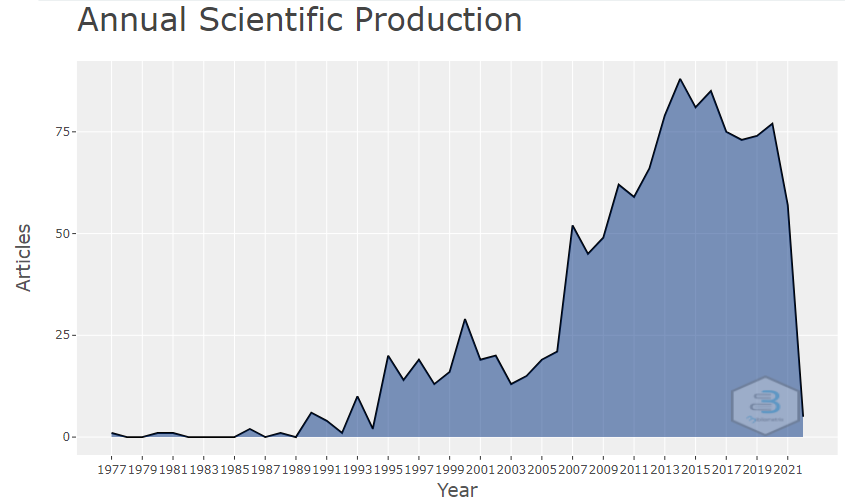
\includegraphics[width=1\textwidth]{experiments/MoustacheGolem/T1/img1AnnualScientifiProduction.PNG}%img1
    \caption{Evolução da produção científica no DSF.}
    \label{fig:evol:anual:DSF@MoustacheGolem}
\end{figure}


A figura \ref{fig:evol:anual:DSF@MoustacheGolem} apresenta a evolução da produção científica mundial no tema de interesse, segundo o DSF. A curva mostra uma tendência de crescimento aproximadamente exponencial da quantidade de publicações, com aceleração mais pronunciada no inicio dos anos 90, mas com uma queda que obteve inicio em 2016.

O \textit{Annual Growth Rate} do dataset   é de 4.45\%, é ligeiramente  maior que \newline a taxa média de crescimento da publicação científica mundial, de cerca de 3,3\% anuais, em 2016, como ilustra o estudo em: \newline \url{https://www.researchgate.net/publication/333972683_Dynamics_of_scientific_production_in_the_world_in_Europe_and_in_France_2000-2016}, página 23.
\newpage
\subsection{Interpretação do Crescimento} A taxa de crescimento do DSF, é relativamente mundana, mais interessante é observar a queda no numero de artigos depois de 2015, possivelmente influenciada por mudanças de interesse politicas e o advento da pandemia.


\subsection{Evolução das Citações}

\begin{figure}
    \centering
    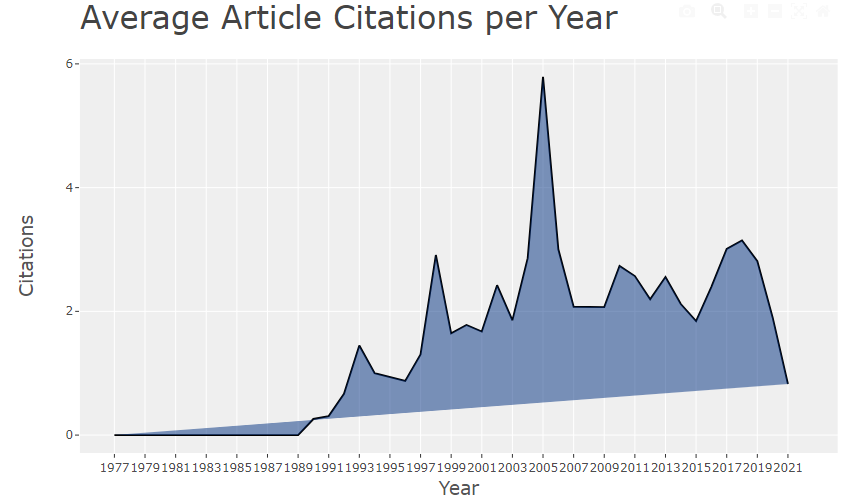
\includegraphics[width=1\textwidth]{experiments/MoustacheGolem/T1/img2AvarageArticleCitationsPerYear.PNG}%img2
    \caption{Evolução da produção científica noDSF.}
    \label{fig:evol:citacoes:DSF@MoustacheGolem}
\end{figure}


A figura \ref{fig:evol:citacoes:DSF@MoustacheGolem} apresenta a evolução das citações dos artigos no tema de interesse, segundo o DSF. A curva mostra  crescimento bem inconsistente  desde a primeira identificada em 1977.

O pico observado no ano de 2005 deve-se, possivelmente, à presença de um artigo famoso, publicado em 2005, que possui um número surpreendente grande de citações, outros artigos famosos mas não no mesmo nível  são observados em outros anos. 

\subsection{Interpretação das Citações}
O relativo crescimento do numero de citações mostra que é possível que o campo de estudo tenha obtido mais relevância ao longo do tempo.
%%%%%%%%%%%%%%%%%%%%%%%%%%%%%%%%%%%%%%%%%%%%%%%%%%%%%%%%%%
\subsection{\textit{Three-Field Plots (Sankey diagram)}}

As \textit{Three-Field Plots (Sankey diagram)} (plotagens do tipo ``Três Campos'') apresentam afinidades entre três conjuntos de atributos agregados que ocorrem no dataset. Uma plotagem do tipo Sankey busca mostrar os principais fluxos entre diferentes conjuntos de itens. 

\begin{figure}
    \centering
    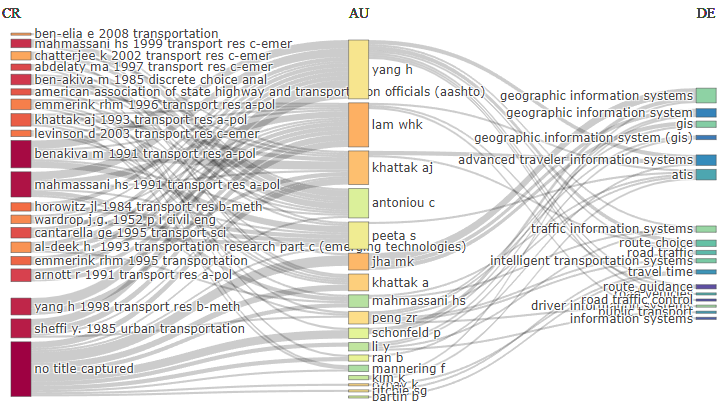
\includegraphics[angle=0,width=0.8\textwidth]{experiments/MoustacheGolem/T1/img3ThreeFieldsPlot.PNG}%img3
    \caption{Plotagem ``Três Campos'' (Sankey plot) do DSF: 20 Autores, Citações e Palavras-Chave mais proeminentes.}
    \label{fig:ThreeFieldPlot:DSF@MoustacheGolem}
\end{figure}


A figura \ref{fig:ThreeFieldPlot:DSF@MoustacheGolem} apresenta a plotagem do tipo ``Três Campos'' do BDF, vinculando, ao centro, os 20 Autores mais proeminentes (AU), à esquerda, as 20 Citações mais frequentes (CR - Cited Records), e à direita, as 20 Palavras-Chave mais frequentes empregadas pelos autores.

\subsection{Interpretação da figura \ref{fig:ThreeFieldPlot:DSF@MoustacheGolem}}
Os vinte autores mais relevantes, em relação aos artigos mais relevantes citados, e as palavras-chave mais relevantes são aparentemente de origem variada, mas com nomes chinesa ocupando bastante espaço. Isso se deve, provavelmente, a grande contribuição chinesa no geral, não a qual quer relevância especifica a nosso campo de estudo.

Dentre as palavras-chave (DE) não relacionadas diretamente aos termos de busca, emergem os principalmente os termos \textbf{geografic information sistemas} e suas formas de escrita similares, e \textbf{Adcanced traveler information systems} e suas variações.Isso sugere que o foto do campo esta muito ligado a desenvolvimento de tecnologias envolvidas com GPS, e sistemas similares.


\subsection{Clustering by coupling}

\begin{figure}
    \centering
    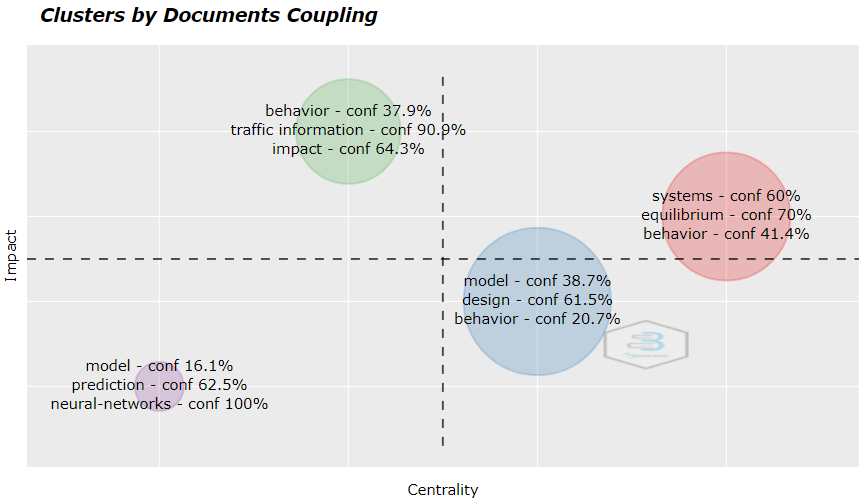
\includegraphics[width=0.7\textwidth]{experiments/MoustacheGolem/T1/img4ClusterByDocumentsCoupling.PNG}%img4
    \caption{Cluster by coupling}
    \label{fig:evol:Clusters:DSF@MoustacheGolem}
\end{figure}

A figura \ref{fig:evol:Clusters:DSF@MoustacheGolem} apresenta o clustering by coupling, ou cluster por acoplamento, que nos mostra os campos de estudos mais relevantes levando em conta comparações feitas conectando termos frequente, podemos observar os campos de mais relevância,   \textbf{trafic information} obviamente, \textbf{equilibrium} e \textbf{prediction}.
\newpage
\subsection{Documentos Mais Citados Glovalmente.}

\begin{figure}
    \centering
    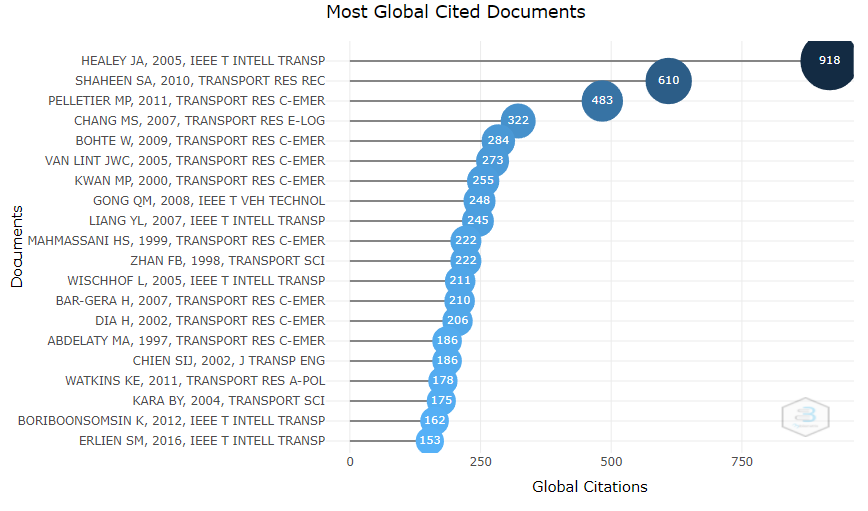
\includegraphics[width=1\textwidth]{experiments/MoustacheGolem/T1/img5MostGlobalCitedDocuments.PNG}%img5
    \caption{Os 20 artigos mais citados globalmente.}
    \label{fig:evol:MaisCita:DSF@MoustacheGolem}
\end{figure}


Em \ref{fig:evol:MaisCita:DSF@MoustacheGolem} Temos os 20 artigos do DSF mais citados globalmente, observaremos os 3 mais citados.

\begin{enumerate}
\item Detecting stress during real-world driving tasks using physiological sensors.
\small\textit{This paper presents methods for collecting and analyzing physiological data during real-world driving tasks to determine a driver's relative stress level. Electrocardiogram, electromyogram, skin conductance, and respiration were recorded continuously while drivers followed a set route through open roads in the greater Boston area. Data from 24 drives of at least 50-min duration were collected for analysis. The data were analyzed in two ways. Analysis I used features from 5-min intervals of data during the rest, highway, and city driving conditions to distinguish three levels of driver stress with an accuracy of over 97\% across multiple drivers and driving days. Analysis II compared continuous features, calculated at 1-s intervals throughout the entire drive, with a metric of observable stressors created by independent coders from videotapes. The results show that for most drivers studied, skin conductivity and heart rate metrics are most closely correlated with driver stress level. These findings indicate that physiological signals can provide a metric of driver stress in future cars capable of physiological monitoring. Such a metric could be used to help manage noncritical in-vehicle information systems and could also provide a continuous measure of how different road and traffic conditions affect drivers.};

\item BIKESHARING IN EUROPE, THE AMERICAS, AND ASIA:
PAST, PRESENT, AND FUTURE.
\small\textit{Growing concerns over global motorization and climate change have led to increasing interest in
sustainable transportation alternatives, such as bikesharing (the shared use of a bicycle fleet).
Since 1965, bikesharing has grown across the globe on four continents including: Europe, North
America, South America, and Asia (including Australia). Today, there are approximately 100
bikesharing programs operating in an estimated 125 cities around the world with over 139,300
bicycles. Bikesharing’s evolution is categorized into three generations: 1) White Bikes (or Free
Bike Systems); 2) Coin-Deposit Systems; and 3) IT-Based Systems. In this paper, the authors
propose a fourth-generation: “Demand-Responsive, Multi-Modal Systems.” A range of existing
bikesharing business models (e.g., advertising) and lessons learned are discussed including: 1)
bicycle theft and vandalism; 2) bicycle redistribution; 3) information systems (e.g., real-time
information); 4) insurance and liability concerns; and 5) pre-launch considerations. While limited
in number, several studies have documented bikesharing’s social and environmental benefits
including reduced auto use, increased bicycle use, and a growing awareness of bikesharing as a
daily mobility option. Despite bikesharing’s ongoing growth, obstacles and uncertainty remain,
including: future demand; safety; sustainability of business models; limited cycling
infrastructure; challenges to integrating with public transportation systems; technology costs; and
user convenience (e.g., limited height adjustment on bicycles, lack of cargo space, and exposure
to weather conditions). In the future, more research is needed to better understand bikesharing’s
impacts, operations, and business models in light of its reported growth and benefits}

\item Smart card data use in public transit: A literature review
\small\textit{Smart card automated fare collection systems are being used more and more by public transit agencies. While their main purpose is to collect revenue, they also produce large quantities of very detailed data on onboard transactions. These data can be very useful to transit planners, from the day-to-day operation of the transit system to the strategic long-term planning of the network. This review covers several aspects of smart card data use in the public transit context. First, the technologies are presented: the hardware and information systems required to operate these tools; and privacy concerns and legal issues related to the dissemination of smart card data, data storage, and encryption are addressed. Then, the various uses of the data at three levels of management are described: strategic (long-term planning), tactical (service adjustments and network development), and operational (ridership statistics and performance indicators). Also reported are smart card commercialization experiments conducted all over the world. Finally, the most promising research avenues for smart card data in this field are presented; for example, comparison of planned and implemented schedules, systematic schedule adjustments, and the survival models applied to ridership.}


O primeiro artigo usa sistemas de informação para coletar e conectar dados fisiológicos de motoristas e conectar a dados no transito.

O segundo foca no conceito de \textit{bikesharing}, observa resultados sobre como usar bicicletas usadas por varias pessoas.

E o terceiro em informação em como utilizar \textit{smartcats} cartões espertos como passes de transporte recarregáveis designados a uma pessoa especifica, e as informações que eles podem coletar.

O foque é bem variado, mas esses árticos mais citados, principalmente o primeiro e segundo, estão exatamente no campo que queremos estudar, mas o primeiro, mostra caminhos para aprimorar nossa query, não necessariamente para eliminar artigos não relevantes mas para especificar mais nosso campo de estudo, Talvez focando em sistemas de informação em transporte públicos.
\end{enumerate}
%%%%%%%%%%%%%%%%%%%%%%%%%%%%%%%%%%%%%%%%%%%%%%%%%%%%%%%%%%
\section{Conclusões}
O termo sistemas de informação, da maneira que é entendido atualmente, é relativamente novo, foi necessário a evolução de hardware até o ponto onde manipular grande quantia de informação era possível, o que explica a timeline do surgimento de artigos, pois estudos com o outro lado do tema, transporte, existe a milênios.

Foi interessante observar como variado os estudos são, era esperado achar estudos girando muito em torno do uso de tecnologias geográficas e IA para mapeamento, mas fui surpreendente achar uso de sistemas de informação para monitorar respostas e emoções de motoristas , o que vai muita além de apenas observar movimento.

Infelizmente os estudos observados continuam muito abrangentes, seria necessário engajar com outras rodadas de aprimoramento de query para não só aprimorar resultados mas focar em algo mais especifico, mas confesso que esse assunto se mostrou desinteressante no geral e dado tempo mudaria o foco completamente.

%%%%%%%%%%%%%%%%%%%%%%%%%%%%%%%%%%%%%%%%%%%%%%%%%%%%%%%%%%
